%%%%%%%%%%%%%%%%%%%%%%%%%%%%%%%%%%%%%%%%%%%%%%%%%%%%%%%%%%%%%%%%%%
%
% Analysis of Algorithms
%
% Homework Assignment #6
%
%%%%%%%%%%%%%%%%%%%%%%%%%%%%%%%%%%%%%%%%%%%%%%%%%%%%%%%%%%%%%%%%%%
%%%%%%%%%%%%%%%%%%%%%%%%%%%%%%%%%%%%%%%%%%%%%%%%%%%%%%%%%%%%%%%%%%
%
% Score Card and Answer Sheets
%
%%%%%%%%%%%%%%%%%%%%%%%%%%%%%%%%%%%%%%%%%%%%%%%%%%%%%%%%%%%%%%%%%%
\documentclass[addpoints,11pt]{exam}
\usepackage{clrscode4e}
\usepackage{tcucosc}
\usepackage{units}
\usepackage{enumitem}
\usepackage{hyperref}
\usepackage{fullpage}
\usepackage{tkz-berge}
\usepackage{graphicx}


%%%%%%%%%%%%%%%%%%%%%%%%%%%%%%%%%%%%%%%%%%%%%%%%%%%%%%%%%%%%%%%%%%
%
% Begin Document
%
%%%%%%%%%%%%%%%%%%%%%%%%%%%%%%%%%%%%%%%%%%%%%%%%%%%%%%%%%%%%%%%%%%
\begin{document}
\pagestyle{empty}


\noindent{\large\bfseries Name: Sabyasachi Sahoo}\\
\noindent{\large\bfseries COSC 40403 - Analysis of Algorithms: Fall 2017: Homework 6}\\
\noindent{\large\bfseries Due: 23:59:59 on November 9, 2018}

%%%%%%%%%%%%%%%%%%%%%%%%%%%%%%%%%%%%%%%%%%%%%%%%%%%%%%%%%%%%%%%%%%
%
% Score Card and Answer Sheets
%
% Comment out one-or-the-other to show or not-show the answers.
%
%%%%%%%%%%%%%%%%%%%%%%%%%%%%%%%%%%%%%%%%%%%%%%%%%%%%%%%%%%%%%%%%%%
\printanswers
%%\noprintanswers


%%%%%%%%%%%%%%%%%%%%%%%%%%%%%%%%%%%%%%%%%%%%%%%%%%%%%%%%%%%%%%%%%%
%
% Score Card
%
%%%%%%%%%%%%%%%%%%%%%%%%%%%%%%%%%%%%%%%%%%%%%%%%%%%%%%%%%%%%%%%%%%
\ifprintanswers
\noindent
\begin{center}
	\gradetable[v][questions]
\end{center}
\newpage
\fi


%%%%%%%%%%%%%%%%%%%%%%%%%%%%%%%%%%%%%%%%%%%%%%%%%%%%%%%%%%%%%%%%%%
%
% Question 1
%
%%%%%%%%%%%%%%%%%%%%%%%%%%%%%%%%%%%%%%%%%%%%%%%%%%%%%%%%%%%%%%%%%%
\begin{questions}
\question[10]
Use Prim's algorithm to find a minimum spanning tree for the following graph.  Show the actions step by step.

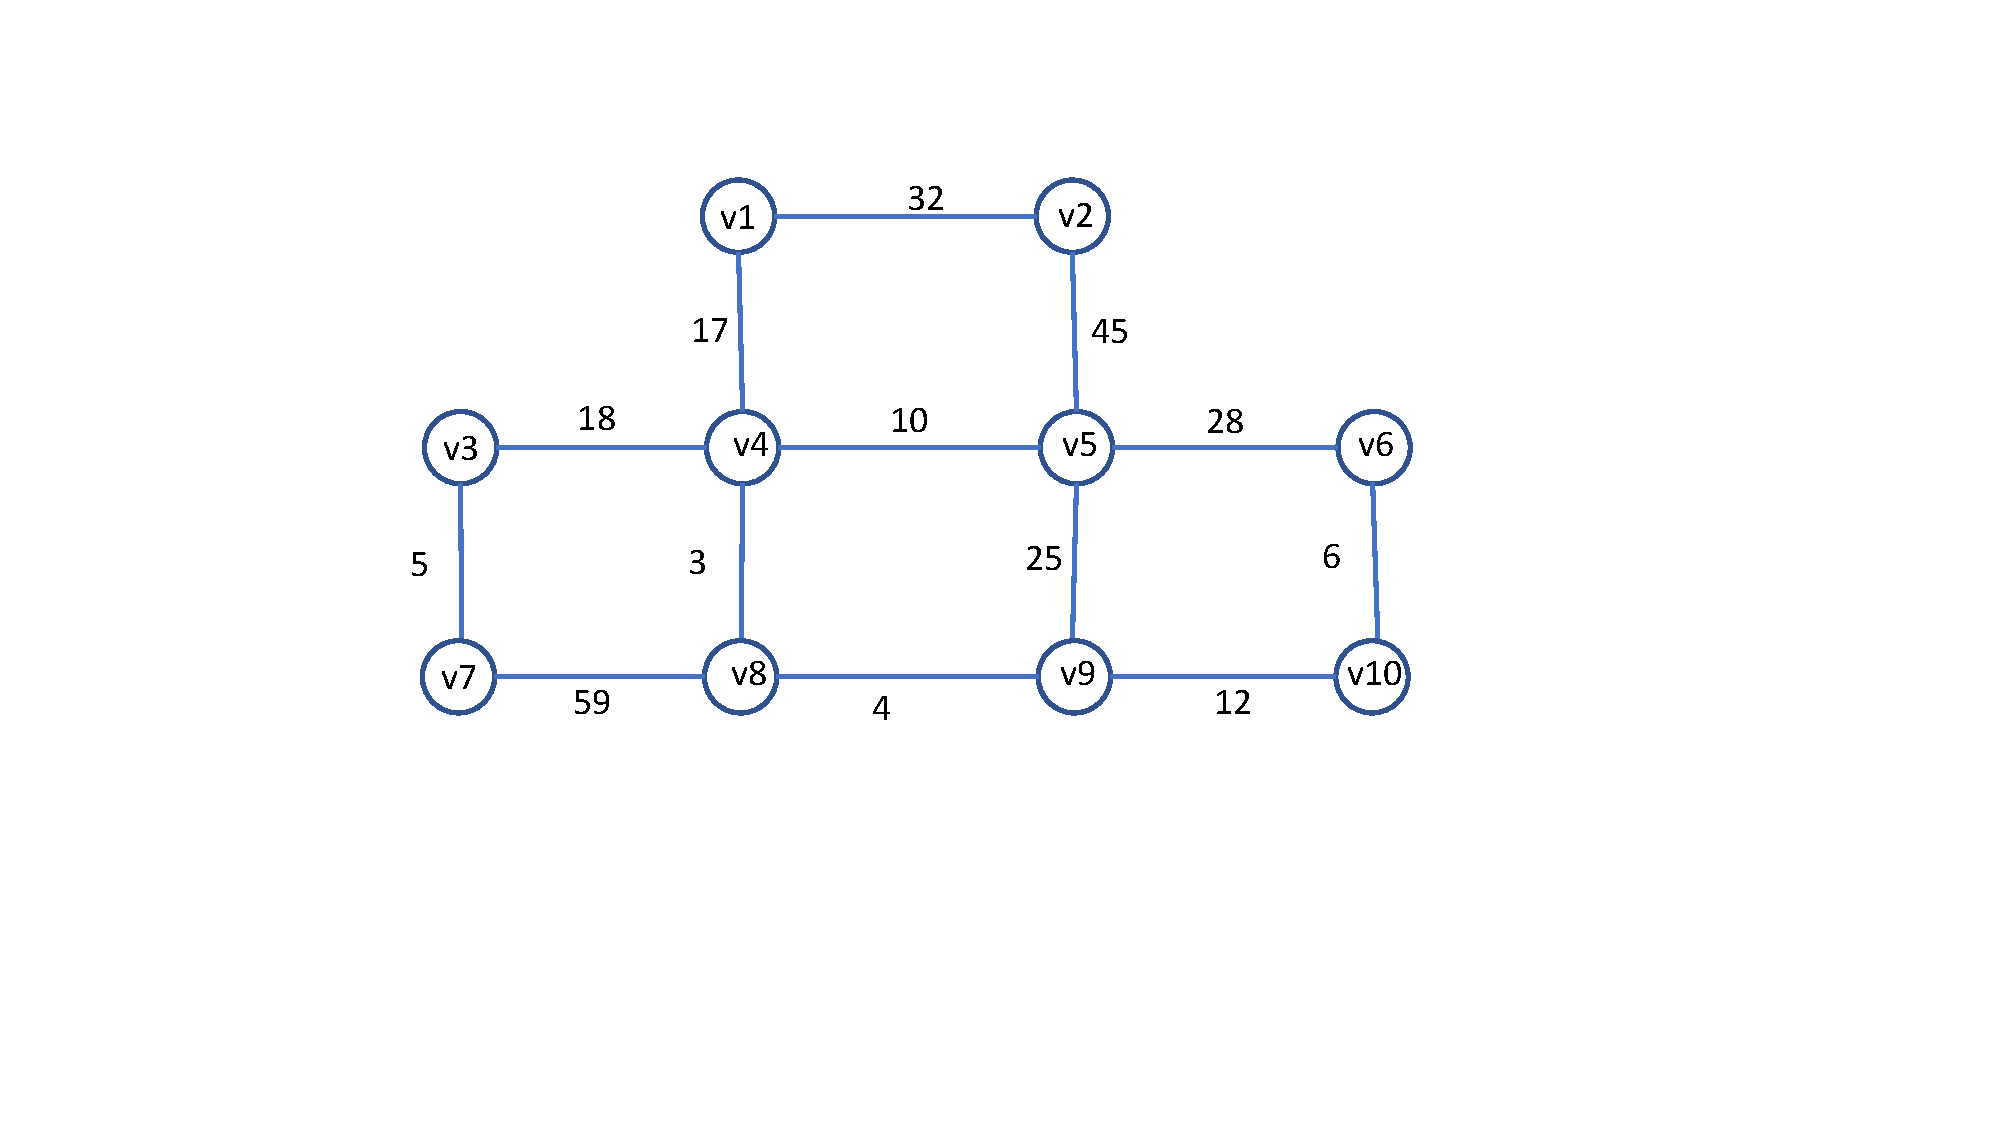
\includegraphics[scale=0.5]{g1.pdf}
\begin{solutionorbox}
\\
Step 1 : No self loops or parallel edges, hence do nothing. \\
\\
Step 2 : Choose any arbitrary note as root node. \\
we select v1.\\
\\
Step 3 : Check outgoing edges and select the one with less cost. \\
\\
$\hspace{15pt}$ Added - (v1, v4) = 17\\
$\hspace{15pt}$ Added - (v4, v8) = 3\\
$\hspace{15pt}$ Added - (v8, v9) = 4\\
$\hspace{15pt}$ Added - (v4, v5) = 10\\
$\hspace{15pt}$ Added - (v9, v10) = 12\\
$\hspace{15pt}$ Added - (v10, v6) = 6\\
$\hspace{15pt}$ Added - (v4, v3) = 18\\
$\hspace{15pt}$ Added - (v3, v7) = 5\\
$\hspace{15pt}$ Added - (v1, v2) = 32\\

Hence,  the list of added edges is the MST produced by Kruskal's algorithm.
\end{solutionorbox}

\ifprintanswers
\newpage
\else
\bigskip
\fi


%%%%%%%%%%%%%%%%%%%%%%%%%%%%%%%%%%%%%%%%%%%%%%%%%%%%%%%%%%%%%%%%%%
%
% Question 2
%
%%%%%%%%%%%%%%%%%%%%%%%%%%%%%%%%%%%%%%%%%%%%%%%%%%%%%%%%%%%%%%%%%%
\question[10]
Use Kruskal's algorithm to find a minimum spanning tree for the graph shown above.  Show the actions step by step.

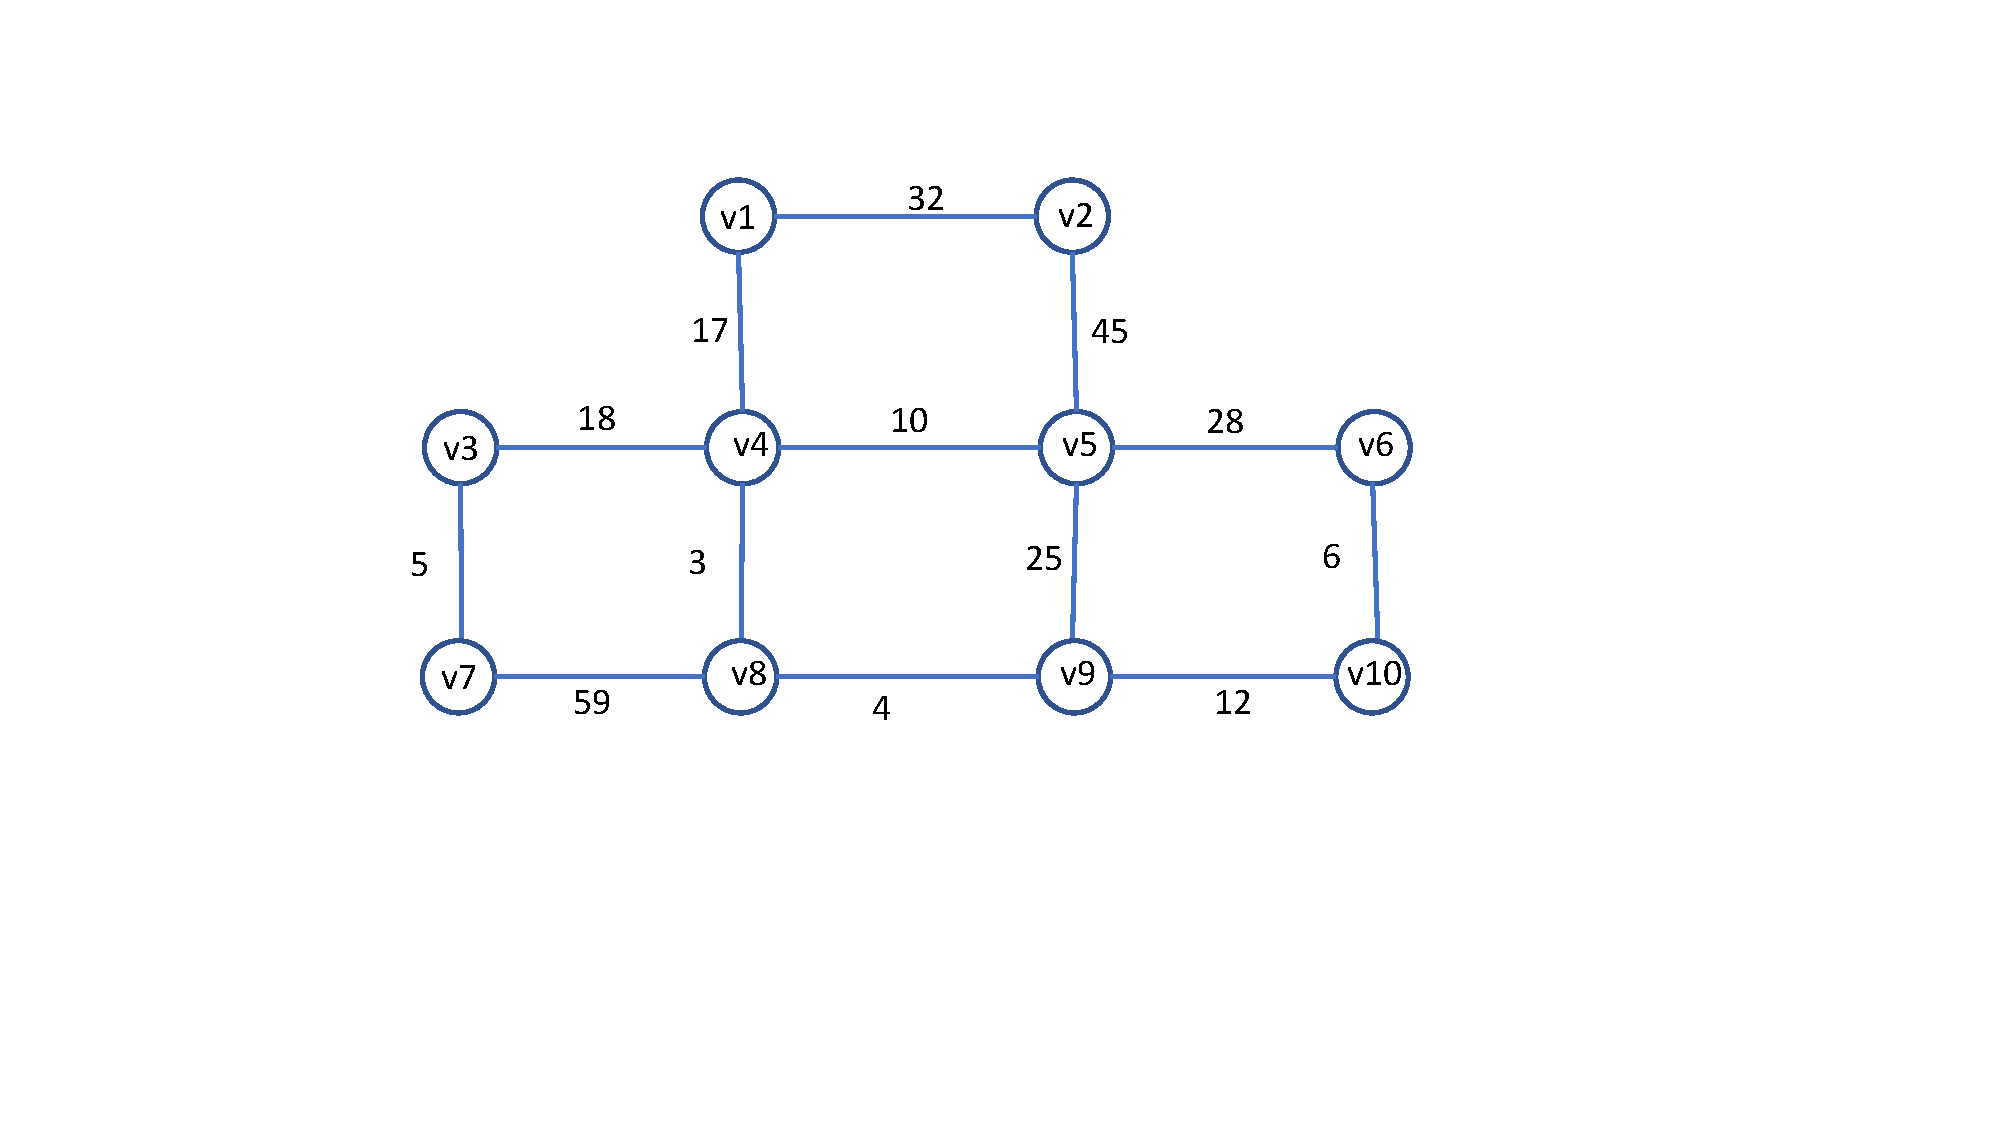
\includegraphics[scale=0.5]{g1.pdf}
\begin{solutionorbox}
Step 1 : No self loops or parallel edges, hence do nothing. \\
\\
Step 2 : Arrange all edges in their increasing order of weight. \\
\\
 $\hspace{15pt}$ (v4, v8) = 3\\
 $\hspace{15pt}$ (v8, v9) = 4\\
 $\hspace{15pt}$ (v3, v7) = 5\\
 $\hspace{15pt}$ (v6, v10) = 6\\ 
 $\hspace{15pt}$ (v4, v5) = 10\\
 $\hspace{15pt}$ (v9, v10) = 12\\
 $\hspace{15pt}$ (v1, v4) = 17\\
$\hspace{15pt}$ (v3, v4) = 18\\
$\hspace{15pt}$ (v5, v9) = 25\\
$\hspace{15pt}$ (v5, v6) = 28\\
$\hspace{15pt}$(v1, v2) = 32\\
$\hspace{15pt}$ (v2, v5) = 45\\
$\hspace{15pt}$ (v7, v8) = 59\\



Step 3 : Add the edge which has the least weightage while keeping the MST property intact. 

 Added - (v4,v8) = 3\\
$\hspace{15pt}$ Added - (v8, v9) = 4\\
$\hspace{15pt}$ Added - (v3, v7) = 5\\
$\hspace{15pt}$ Added - (v10, v6) = 6\\
$\hspace{15pt}$ Added - (v4, v5) = 10\\
$\hspace{15pt}$ Added - (v9, v10) = 12\\
$\hspace{15pt}$ Added - (v1, v4) = 17\\
$\hspace{15pt}$ Added - (v3, v4) = 18\\
$\hspace{15pt}$ (v5, v9) and (v5, v6) aren't added as they create circuits \\
$\hspace{15pt}$ Added - (v1, v2) = 32\\
$\hspace{15pt}$ (v2, v5) and (v7, v8) aren't added as they create circuits \\

Hence,  the list of added edges is the MST produced by Kruskal's algorithm.

\end{solutionorbox}

\ifprintanswers
\newpage
\else
\bigskip
\fi


%%%%%%%%%%%%%%%%%%%%%%%%%%%%%%%%%%%%%%%%%%%%%%%%%%%%%%%%%%%%%%%%%%
%
% Question 3
%
%%%%%%%%%%%%%%%%%%%%%%%%%%%%%%%%%%%%%%%%%%%%%%%%%%%%%%%%%%%%%%%%%%
\question[10]
Use Huffman's algorithm to construct an optimal binary prefix code for the letters in the following table.

\begin{tabular}{|c|c|c|c|c|c|c|c|}
	\hline
	Letter    & c    & e    & i    & r    & s    & t    & x    \\ \hline
	Frequency & 0.11 & 0.22 & 0.16 & 0.12 & 0.15 & 0.10 & 0.14 \\ \hline
\end{tabular}

Encode each word using your binary code.
\begin{enumerate}
	\item rise
	\item exit
	\item text
	\item exercise
\end{enumerate}

\begin{solutionorbox}
\\
Symbol -- Huffman Encoding \\
e -- 01\\
c -- 001\\
i -- 111\\
r -- 100\\
s -- 110\\
t -- 000\\
x -- 101\\

rise: 10011111001\\
exit: 01101111000\\
text: 00001101000\\
exercise: 011010110000111111001\\
\end{solutionorbox}

\ifprintanswers
\newpage
\else
\bigskip
\fi

%%%%%%%%%%%%%%%%%%%%%%%%%%%%%%%%%%%%%%%%%%%%%%%%%%%%%%%%%%%%%%%%%%
%
% Question 4
%
%%%%%%%%%%%%%%%%%%%%%%%%%%%%%%%%%%%%%%%%%%%%%%%%%%%%%%%%%%%%%%%%%%
\question[15]
Implement Huffman's algorithm using Python and run it on problem 3.
\begin{solutionorbox}
 Jupiter notebook attached in the zip file.
\end{solutionorbox}

\ifprintanswers
\newpage
\else
\bigskip
\fi




\end{questions}
\end{document}
